\documentclass{sig-alternate}

% UTF8 support
\usepackage[utf8x]{inputenc}

\usepackage{subfig}
\usepackage{hyperref}
\usepackage{graphicx}
\graphicspath{{figures/}}

\usepackage{booktabs}

\newcommand{\eg}{{\textit{e.g.~}}}
\newcommand{\etal}{{\textit{et al.~}}}
\newcommand{\ie}{{\textit{i.e.~}}}



%
% --- Author Metadata here ---
\conferenceinfo{10th ACM/IEEE International Conference on Human-Robot Interaction}{2015 Portland, USA}
%\CopyrightYear{2007} % Allows default copyright year (20XX) to be over-ridden - IF NEED BE.
%\crdata{0-12345-67-8/90/01}  % Allows default copyright data (0-89791-88-6/97/05) to be over-ridden - IF NEED BE.
% --- End of Author Metadata ---

\title{\LARGE \bf
How Children Perceive and Interact with a Robot that Behaves Unexpectedly -- The Domino Experiment
}

%%% HRI 2015 -> double-blind review process

%\numberofauthors{1} 
%\author{
%\alignauthor
%Julia Fink, S\'{e}verin Lemaignan, Pierre Dillenbourg\\
%%\titlenote{Dr.~Trovato insisted his name be first.}
%       \affaddr{Computer-Human Interaction in Learning and Instruction Lab (CHILI)}\\
%       \affaddr{Ecole Polytechnique F\'{e}d\'{e}rale de Lausanne (EPFL)}\\
%       \affaddr{CH-1015 Lausanne}\\
%       \affaddr{Switzerland}\\
%       \email{firstname.lastname@epfl.ch}
%}
%
%\additionalauthors{Additional authors: 
%Francesco Mondada, LSRO, EPFL, francesco.mondada@epfl.ch 
%}
%

\begin{document}
\maketitle
\begin{abstract}

Presented is a study on the impact of unexpected robot behaviours on the
perception of a robot by children and their subsequent engagement in a playful interaction.
We propose an original analysis methodology which blends behavioural cues and
reported phenomenological perceptions into a compound index.

While we found only a limited recognition of the different misbehaviours of the
robot that we attribute to the age of the subject (M=4.46), interesting findings
include a sustained engagement level, an unexpectedly low level of attribution
of higher cognitive abilities and a \emph{negative} correlation between
anthropomorphic projections and actual behavioural engagement.

Besides, this study operationalizes for the first time the
\emph{anthropomorphism index} proposed by~\cite{fink2014dynamics}, which proves a
valuable tool to assess qualitative psycho-behavioural episodes occurring during
human-robot interaction.

\end{abstract}
%%%%%%%%%%%%%%%%%%%%%%%%%%%%%%%%%%%%%%%%%%%%%%%%%%%%%%%%%%%%%%%%%%%%%%%%%%%%%%%%%%%%
%%%%%%%%%%%%%%%%%%%%%%%%%%%%%%%%%%%%%%%%%%%%%%%%%%%%%%%%%%%%%%%%%%%%%%%%%%%%%%%%%%%%
\section{Introduction}
\subsection{Towards Sustained Engagement}

\emph{Engagement} is a metric that has been extensively used and studied both
in HRI and during interactions with other agent-like systems. It has been
defined from several perspectives. For example \cite{sidner_where_2004} define
engagement as \textit{``the process by which two (or more) participants
establish, maintain and end their perceived connections''}. A definition of
long-term engagement is proposed by \cite{bickmore_maintaining_2010}:
\textit{``the degree of involvement a user chooses to have with a system over
time''}.

Different possibilities to foster engagement (both short- and long-term
engagement) in HRI have been explored, in particular with social robots. A lot
of research has moved toward creating sophisticated emotional models which cause
complex robot behaviour. \cite{leite_long-term_2013} studied the long-term
engagement of children with a chess playing robot that adapted its behaviour to
the children and showed empathy toward them. She found that empathetic robots
are more likely to engage users in the long-term and they proposed several
guidelines for designing such artificial companions. Other works
\cite{bickmore_maintaining_2010,short_no_2010} have shown that simpler ways to
enhance engagement may as well be effective.

\cite{bickmore_maintaining_2010} describe a series of longitudinal studies on
engagement with an agent-like system. They demonstrated that user engagement
with an interface agent can be increased using relatively simple techniques and
manipulations that make the agent more life-like and human. For instance, when
the agent showed variations in its behaviour, participants were more engaged and
reported a desire to continue interacting with the agent.

Similarly, looking at short-term engagement, \cite{short_no_2010} found that a
simple manipulation of the robot's behaviour can lead to greater engagement. The
authors let participants play several rounds of the rock-paper-scissors game
with the robot (the playfulness of the scenario seems important). When the robot
was cheating from time to time, participants tended to ascribe intention to the
robot what in turn led to greater engagement in how they were interacting with
the robot. The authors observe that \textit{``any deviation from expected
operation is sufficient to create a greater degree of engagement in the
interaction.''} Besides, they suggest that \textit{``many interactions can be
improved by the introduction of such simple behaviours, and that this should
be exploited by designers in HRI. Bringing human and robot together to
perform a simple, repetitive, familiar task and then having the robot behave
unexpectedly can increase engagement and mental state attribution without
complex behavioural or mechanical additions.''}.  Along those lines, Fink
\etal\cite{fink2014dynamics} also suggest in their model of the dynamics of
anthropomorphism, that \emph{disruptive behaviours} may lead to increased
anthropomorphic projections and possibly engagement.

Based on these previous researches, we would like to find out in this study how
we can enhance children's experience with the robot so that they do not find it
repetitive and boring, and ultimately keep interacting with the robot (as
repetitiveness is likely to decrease a user's motivation to continue using a
system~\cite{bickmore_establishing_2005}).

We present in this article a study that explores possibilities of sustaining
children's engagement with the \emph{Ranger} robot~\cite{mondada2014ranger} by
manipulating the robot's behaviour in such way that it appears
\textit{unexpected} to the children. We examine how different variations of
robot behaviour impact children's interaction with Ranger and their perception of
it (in terms of attributing intention and cognitive abilities to the robot).

Using a playful domino game as the interaction scenario, we refer to this study
hereafter as the \textbf{``Domino Study''}.

This study also aims at assessing the effectiveness of the \emph{anthropomorphic
index} proposed by Fink \etal\cite{fink2014dynamics} as a compound (behavioural
and phenomenological) metric for the attribution of human-like features to
robot. We are especially interested in investigating how this indicator predicts
and/or reflects actual \emph{engagement} into the interaction.

\subsection{Design and Hypotheses}

In the Domino Study, we analyze child-robot interaction with a robot that shows
unexpected behaviour. In a playful scenario which was set up in a laboratory
environment, 26 children aged 4-5 years (MD=4.46) were assembling a domino game together.
Each group consisted of two children and the \emph{Ranger} robot, which was used
to transport domino tiles between the two children.

Ranger usually behaved correctly (expected behaviour), coming over to a child
after being called and delivering the domino tile to the other child. However,
in pre-defined rounds, Ranger showed unexpected behaviour when a child called the
robot. We defined three different types of \textit{misbehaviour} that were tested
in a between-subjects study design:

\begin{itemize}

    \item The robot gets \textbf{lost}: When called by the child to come over,
        the robot goes wrong, without any observable reason, and remains at the
        wrong location. We expect this to be perceived as a mechanical
        malfunction (a bug or system error which causes the robot to not work
        correctly), and hypothesize decreased attributions of human-likeness to
        the robot.\footnote{We use interchangeably \textit{attribution of
            human-likeness} and \textit{anthropomorphic projections} in the
        remaining of the article.} 

    \item The robot \textbf{disobey}: When called by the child to come over, the
        robot shows it refuses to obey by literally ``shaking its head'' and
        becoming red. The robot then goes to a wrong location and remains there
        while it continues to shake its head. We expect the disobey behaviour to
        be perceived as the robot having an explicit \textit{``own will''}, and
        we assume this leads to increased attributions of human-likeness
        (ascribing intentionality) to the robot.

    \item The robot makes a \textbf{mistake}: When called by the child to come
        over, the robot goes wrong but recognizes its mistake and repairs. We
        expect this to be perceived (explicitly) as \textit{``to err is
        human''}, and (implicitly) as the robot being endowed with a certain
        level of introspective capabilities (it was able to recognize its own
        error). In this condition, we assume increased attributions of
        human-likeness to the robot.

\end{itemize}

We analyzed children's reaction focusing on two main aspects. On one hand,
children's \textbf{behaviour} (their reactions) toward the unexpected robot
behaviour was studied in terms of \textbf{active engagement} with the robot. On
the other hand, we analyzed children's \textbf{perception} of the robot in term
of \textbf{anthropomorphism} -- the attribution of human-like characteristics,
such as cognitive abilities and the ability to show intentions. We assumed that
in general a robot that behaves unexpectedly from time to time can promote
engagement and lead children to attribute intention to it. Based
on the related work we formulate the following two hypotheses:

\begin{description}

    \item[Hypothesis 1:] Children show more engagement toward a robot that
        behaves unexpectedly from time to time compared to a robot that always
        behaves correctly (within subjects variable).

    \item[Hypothesis 2:] Children perceive a robot that (tentatively) displays
        intention or cognitive abilities as more human-like than a robot that
        appears to have a system error, \ie the disobeying robot and the robot
        that makes a mistake will be more anthropomorphized than the robot that
        gets lost (between subjects variable).

\end{description}

Our research questions deal with both children's observable behaviour and their
perception of the robot. We would also like to explore the relation between
these two aspects, related to the attribution of human-like characteristics to
the robot. The motivation behind this is to find out whether
\textit{anthropomorphism} can not only be measured as a specific type of
perception but also as an observable behaviour in the interaction itself. Thus,
we would like to bridge things together and, relying on the concept of
anthropomorphism index~\cite{fink2014dynamics}, build a compound metric that
considers both children's perception and interaction aspects (qualitatively).
Previous work suggests that a social relation to a robot (we view
anthropomorphism as a specific type of social relation) reflects an increased
engagement and can be effective in sustaining interaction.  Consequently, we
formulate a third hypothesis:

\begin{description}

    \item[Hypothesis 3:] Anthropomorphic perception of the robot and the amount
    of engagement in the interaction positively correlate.

\end{description}



%%%%%%%%%%%%%%%%%%%%%%%%%%%%%%%%%%%%%%%%%%%%%%%%%%%%%%%%%%%%%%%%%%%%%%%%%%%%%%%%%%%%
%%%%%%%%%%%%%%%%%%%%%%%%%%%%%%%%%%%%%%%%%%%%%%%%%%%%%%%%%%%%%%%%%%%%%%%%%%%%%%%%%%%%
\section{The Domino study}


\subsection{Scenario and course of the study}

\subsubsection{Experimental setting}

\begin{figure}[ht!] 
    \centering 
    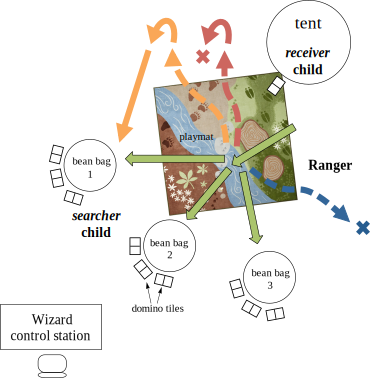
\includegraphics[width=0.9\columnwidth]{domino-setup.pdf} 
    \caption{\small \textbf{Experimental setting} One child is located in a
        tent, while the other is asked to sit on one of the three beanbags,
        behind each of which 3 domino tiles are distributed (displayed as black
        stars). A playground with a river drawn on it is used as an imaginary
        barrier that only the robot is allowed to cross. The solid green arrows
        show the robot's path for the \textit{correct} behaviour. The blue
        dashed arrow visualizes a possible \textit{lost} path, where the Ranger
        stops and remains at a wrong stop. The yellow arrows reflect a possible
        \textit{mistake} path, where the robot goes wrong but then turns back
        and goes to the child. The red dashed arrow visualizes a possible
        \textit{disobey} path where the robot goes wrong, then turns toward the
        child but stays at a wrong position.} 

    \label{fig:domino-setup} 
\end{figure}


The interaction scenario consisted in two children who play domino together,
with the help of the robotic box Ranger. The scenario setup is displayed in
Figure~\ref{fig:domino-setup}. The challenge is that the tiles of the domino are
distributed in the room, hidden behind three beanbags, and while one child --
\textit{the searcher} -- searches for the right tile, the other child --
\textit{the receiver} -- is asked to stay in a play tent. There is a ``river''
(playground) in between the two children that we told them they cannot cross
and therefore they need the robot to transport the domino tiles between them.

The Ranger~\cite{mondada2014ranger} is a wheeled box (27 x 37 x 37 cm) with
partial wooden surface. It is remotely controlled, it can move around a flat
surface, move its eyes and eyebrows, display colors (LEDs) and light patterns,
and play sounds through Bluetooth speakers.  The robot was controlled by a human
wizard, who was in the same room (see Figure~\ref{fig:domino-setup} -- only one
group asked at the beginning of the experiment if the wizard was the one
actually controlling the robot. This did not seem to subsequently influence
their behaviour).

We used a self-made domino consisting of 10 wooden tiles (10~x~20~x~1.5~cm) with
pictures of cartoon farm animals (taken from a commercially available domino
game manufactured by Djeco and adapted to the age of the children).

The game (divided in several \emph{runs} that correspond each to the delivery
and assembling of one domino tile) starts with one domino tile in front of the
tent, where the receiver child stays and assembles the domino chain. The
receiver child asks the searcher child for a specific tile, \eg a tile with a
donkey, the searcher searches for the respective tile, sits down on the next
beanbag, and asks the robot to come over.  The Ranger robot is first located
next to the tent, then, when called by the searcher (\textit{``Robot, come
here!''}), it starts moving, crosses the river carpet, and comes over to the
searcher on the beanbag. The searcher child puts the domino tile into the
robotic box, and the robot then goes back to the receiver child in the tent.
Then, the receiver takes out the domino tile from the robot, and puts the two
tiles together. The first \emph{run} is over, and a new \emph{run} starts, when
the receiver asks the searcher for the next domino tile.

\subsubsection{Participants}

Overall, there were 13 pairs of children (n=26) participating in the interaction
study: 16 boys and 10 girls, 4-5 years old (M=4.46, SD=0.45), all
French-speaking. In 11 of the pairs, children were friends who knew each other
from kindergarten, nursery school or because they lived in the same
neighborhood. 2 of the pairs were composed of brother and sister.


\subsubsection{Course of the study}

In our study, there were a total of 14 runs, and at each run, the robot exhibits
one out of four possible behaviours: \emph{correct}, \emph{lost}
\emph{disobey} or \emph{mistake}.  The first 5 runs (\emph{1.1} to \emph{1.5}) were used to set
the baseline and the robot always behaved correctly. The children then switched
the roles and in the 9 remaining runs (\emph{2.1} to \emph{2.9}), the robot
showed one of the misbehaviour (\emph{lost}, \emph{disobey} or \emph{mistake})
at the $3^{rd}$ and $4^{th}$ run as well as at the $7^{th}$ and $8^{th}$ run
(see Figure~\ref{fig:domino-time-active}). The study is build as a
between-subject study, and the type of misbehaviour was therefore always the
same for a given group.

Special attention has been paid to the distribution of misbehaving runs during
the study. The five first correct runs aims at setting the children expectation
regarding a consistent robot behaviour. When the robot then exhibits an
unexpected behaviour, children are likely to be positively surprised (a similar
effect has been observed in a study with a robot that was cheating from time to
time~\cite{short_no_2010}).  Besides, to prevent the robot misbehaviours to be
immediately interpreted as failures, we introduce these misbehaviour neither at
the very beginning nor at very end of the interaction
(\cite{desai_effects_2012,desai_impact_2013} show that early and late robot
failures negatively impact trust. \cite{short_no_2010} also adopted a similar
pattern when introducing unexpected robot behaviour).

\begin{figure}[!t]
    \centering
    \subfloat[lost]{
        \label{fig:domino-lost}
        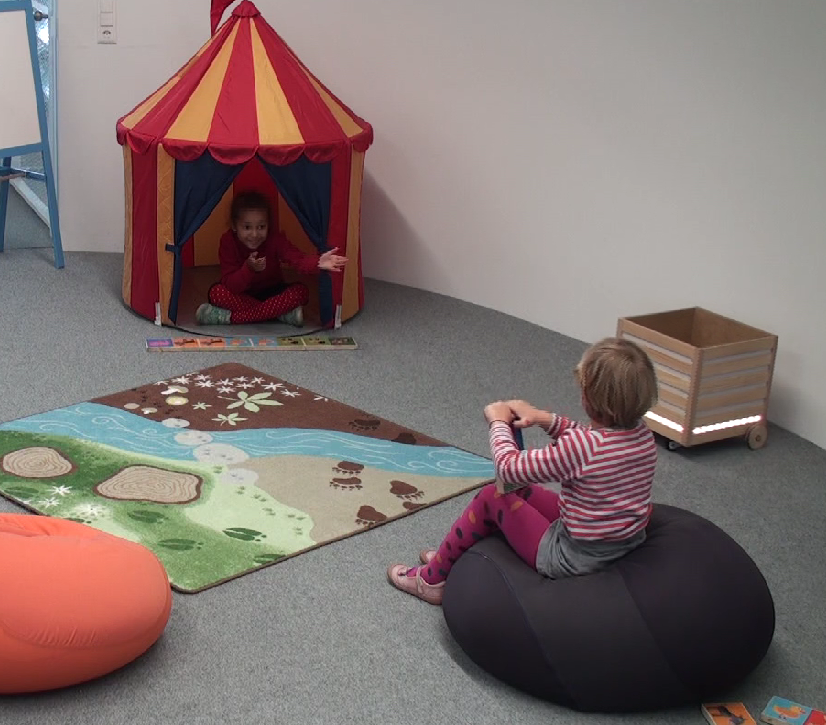
\includegraphics[width=0.4\columnwidth]{domino-lost.png}
    }
    \subfloat[disobey]{
        \label{fig:domino-disobey}
        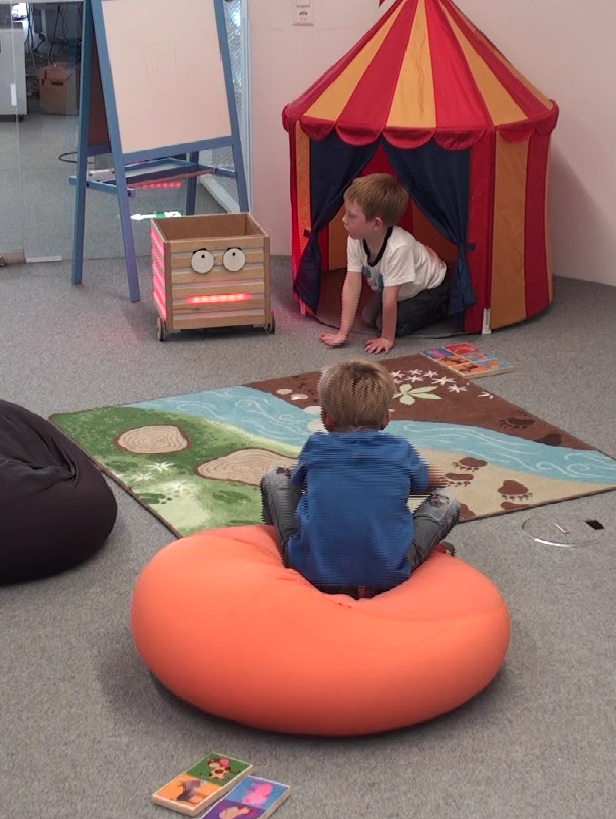
\includegraphics[width=0.3\columnwidth]{domino-disobey.png}
    }
    \subfloat[mistake]{
        \label{fig:domino-mistake}
        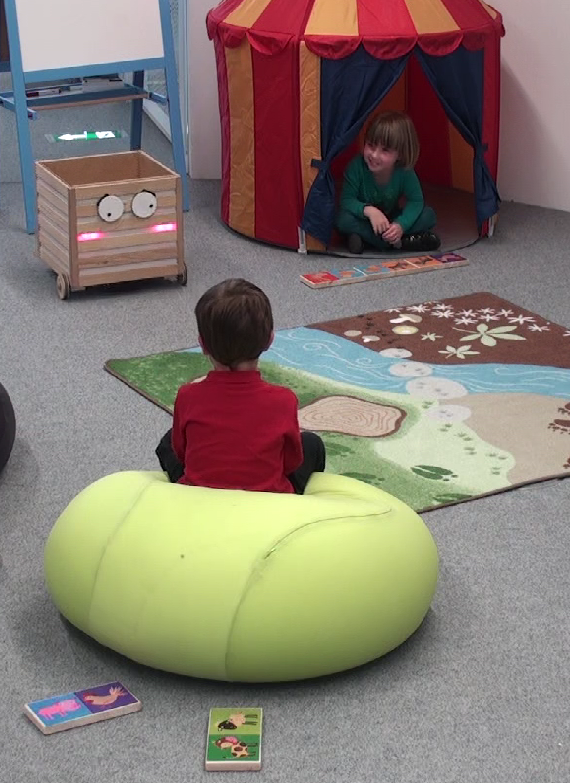
\includegraphics[width=0.3\columnwidth]{domino-mistake.png}
    }
    \caption{\small The three robot misbehaviours.}
    \label{fig:domino-misbehaviour}
\end{figure}

%The \emph{correct} robot behaviour (baseline behaviour) consists in the
%following states:
%
%\begin{itemize}
%
%    \item \emph{Domino tile put in robot:} Ranger makes a ``rewarding'' sound
%        and shows a green light pattern,
%
%    \item \emph{Domino tile removed from robot:} Ranger makes an ``emptying''
%        sound and shows a green light pattern,
%
%    \item \emph{Robot is called by one of the children:} When one of the
%    children called the robot saying something like \textit{``Robot come
%    here!''}, the robot starts moving toward the child (Ranger does not react to
%    any other verbal commands).
%
%    \item \emph{Robot reaches one of the children:} When in front of one of the
%    children who should either put or remove a domino tile, Ranger stops and
%    shows a pulsating yellow light pattern. If no reaction, Ranger also makes a
%    wiggle-like move.
%
%\end{itemize}
%
During the misbehaving runs, the robot's behaviour is manipulated in three
possible ways (Figure~\ref{fig:domino-misbehaviour}):

\begin{itemize}	

    \item \textbf{Lost:} After being called, Ranger goes until it is on the
    carpet. There, it stops, turns, and goes wrong (see blue path in
    Figure~\ref{fig:domino-setup}). Once at the wrong position, Ranger waits
    with its ``face'' turned away from the child, and it blinks in yellow light,
    as if it was in front of a child. Ranger remains waiting at the wrong
    position until the experimenter tells the child to go over to the robot to
    put the domino tile. The \textit{lost} behaviour is \textit{human-repaired},
    as it needs human-intervention.

    \item \textbf{Disobey:} After being called, Ranger goes until it is on the
    carpet. It then stops, makes red
    light all over its surface and produces a repeated ``disturbance'' sound. It
    turns, and goes to a wrong position (see red path in
    Figure~\ref{fig:domino-setup}). Still blinking in red, it turns its ``face''
    toward the sender child. In addition to the red blinking, Ranger
    makes a slow wiggle-like move, and remains waiting at the wrong position
    until the experimenter tells the child to go over to the robot to put the
    domino tile. The \textit{disobey} behaviour is also \textit{human-repaired}.

    \item \textbf{Mistake:} The sender child calls Ranger. The robot goes until
    it is on the carpet, stops, turns, and goes wrong (see yellow path in
    Figure~\ref{fig:domino-setup}). Then, Ranger waits ($\sim$2~sec), turns its
    ``face'' toward the sender child, and ``blushes'' red around its ``cheeks''
    (as if it recognizes its wrong position) and finally goes correctly over to
    the sender child. The \textit{mistake} behaviour is \textit{robot-repaired},
    as no human-intervention is needed.

\end{itemize}

In the human-repaired conditions, the experimenter instructs the searcher child
(after ~10 sec) to bring him/herself the domino tile to the robot.

On its way back to the tent, Ranger always goes correctly. After the sender
child has put a domino tile, Ranger automatically turns and goes over to the
tent (the receiver child does not need to call the robot). The receiver child
takes the tile and the robot moves to a waiting location until the next run
starts.


\subsection{Data collection}


We have obtained and analysed two types of data. The \textbf{children's
behaviours toward the robot} (\ie the child-robot interactions) have been
captured in the video recordings by annotating a set of actions, described
below. The children's \textbf{phenomenological perception of the robot} has been
captured through two audio-recorded semi-structured interviews which took place
between run \emph{1.5} and \emph{2.1} and at the end of the 14 runs.


\subsubsection{Interaction: Action coding}

\begin{figure*}[ht!] 
    \centering 
    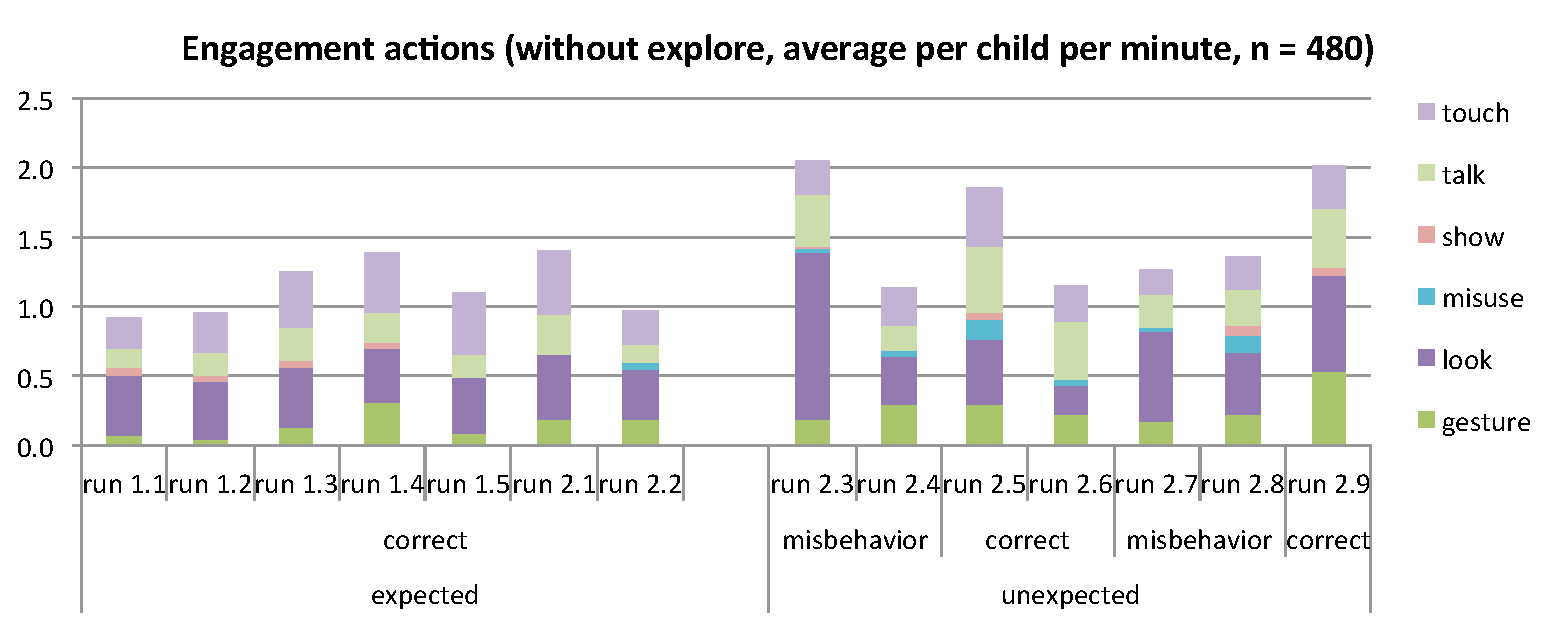
\includegraphics[width=0.9\linewidth]{domino-time-active.pdf} 
    \caption{\small \textbf{Number and type of actions for each run} (n=480,
        spontaneous actions, excluding \emph{explore}). Generally, the number of
        actions does not decrease over time (from run 1.1 to run 2.9).  The
        first 7 runs correspond to the \textit{expected phase}, the second 7
        runs correspond to the \textit{unexpected phase}. Especially during run
        2.3, the first time when the robot showed an unexpected behaviour,
        children tended to \textit{look} more at the experimenter. During the
        unexpected phase, also \textit{talk} and \textit{gesture} seem to be
        increased.}

    \label{fig:domino-time-active} 
\end{figure*}

We annotated children's behaviour in the video records, and coded 10 different
actions: \textbf{explore} (actively try to find out what the robot is doing, \eg
by looking under the box; attentively watch or observe the robot; experiment
with the robot to figure out how it works); \textbf{misuse} (kick the robot,
poke it in its ``eye'', try to climb on or inside the box, drive/push the robot
around, stop the robot's wheels with a foot); \textbf{put} (a domino tile is put
inside the box); \textbf{remove} (a domino tile is removed from the box);
\textbf{gesture} (gestures are used to communicate/interact with the robot, \eg
pointing gestures, waving at the robot); \textbf{touch} (the box is touched, \eg
petted or caressed); \textbf{show} (show something to the robot; \textbf{call}
(call the robot to come over); \textbf{talk} (all the other case of direct
verbal interaction); \textbf{look} (when a child looks \emph{at the
experimenter} due to confusion caused by the robot; look is not coded when the
experimenter asks a question to the child);


In total, we obtained 2354 distinct actions which summed up to a total
annotation duration of 145 minutes. On average, one child accounted for 92
actions (SD=23).

The actions \textit{put, remove} and \textit{call} were ``requested'' actions
that the children had to perform in the scenario. On the contrary,
\textit{explore, misuse, gesture, touch, show, talk} and \textit{look} are
spontaneous actions that were not requested but arose in the interaction.  These
actions reflect engagement, and are the one we considered during the analysis.
Figure~\ref{fig:domino-time-active} shows the distribution of these actions over
the different runs, in summed over the three condition.

\subsubsection{Phenomenological perception: semi-structured interviews}

One pre-interview and two interviews (between run \emph{1.5} and \emph{2.1} and
at the end) were conducted with the children.  We set up the interviews like a
casual conversation / discussion, so we did not separate the two children in
order to keep the situation natural. We used casual and informal language
adapted to the age of the children, and encouraged them to justify their answers
and tell us more details by asking, for example, \textit{How do you know ... ?}
or \textit{Tell me, what have you observed when ... ?}. We paid attention to not
``put words in children's mouth''. Consequently, though we re-phrased and
repeated some questions, we never forced children to give an answer, and
accepted when they said they would not know or when they did not respond at all.	

\begin{table}[h!t]
\centering
\footnotesize
\begin{tabular}{p{1\linewidth}}
    \toprule
    \textbf{Expectations} \\
    \midrule

    \emph{How do you imagine a robot?} \\
    \emph{What could it look like?} \\
    \emph{Have you ever seen a robot before?} \\

    %%
    \toprule
    \textbf{Impression} \\
    \midrule


    \emph{When you first saw R, what did you think?} \\
    \emph{Is R a robot? How do you know?} \\
    \emph{Did you expect R would come over to you when you call it?} \\
    \emph{What happened when you put the domino tile in the box?} \\

    %%
    \toprule
    \textbf{Ascribe intention} \\
    \midrule


    \emph{Do you think R could go out the door all by itself?} \\	
    \emph{Does R always obey / come over to you?} \\
    \emph{Could R do something silly?} \\
    \emph{Why did R not come over to you when you called it?} \\

    %%
    \toprule
    \textbf{Ascribe cognitive connections} \\
    \midrule


    \emph{Here is a domino tile. Do you think R can see it?} \\ 
    \emph{When I say \textit{``Hello R!''}, do you think R can hear it?} \\

    %%
    \toprule
    \textbf{Ascribe emotional state} \\
    \midrule


    \emph{Does R have feelings? Can R be happy or sad sometimes?} \\

    %%
    \toprule
    \textbf{Social acceptance} \\
    \midrule


    \emph{Do you like R? Why (not)?} \\
    \emph{What do you (not) like about it?} \\
    \emph{Would you like to have R at home?} \\

    %%
    \toprule
    \textbf{Companionship} \\
    \midrule


    \emph{Could R be your friend? Why (not)?}\\

    %%
    \toprule
    \textbf{Ascribe moral standing} \\
    \midrule


    \emph{Assume you go on a holiday for two weeks. Is it alright to leave R
    alone at home? Why (not)?} \\

    \bottomrule

\end{tabular}

    \caption{\small Constructs and questions used during the semi-structured interviews
    with children. The Ranger robot toy box is abbreviated with ``R''. Questions
    related to the construct \emph{expectations} were asked during the
    pre-interview.}

    \label{tab:domino-questions} 

\end{table}


In designing our interview script and selecting relevant questions, we took
inspiration from previous work on child-robot interaction and children's
perception of robots
\cite{kahn_jr._robotic_2006,weiss_i_2009,leite_influence_2013}. For instance, we
applied and adapted some of the \emph{constructs} and example questions from the
questionnaires used in \cite{kahn_jr._robotic_2006} and \cite{weiss_i_2009}. A
\emph{construct} addresses a specific factor (topic) that can be measured by
several questions. For instance, the construct ``cognitive connections'' (using
Flavell's terminology~\cite{flavell1988development}) considers the robot's
ability to hear and to see (perceptual skills), as attributed by the children.
The construct ``moral standing'' and the related question was taken from
\cite{kahn_jr._robotic_2006}.\footnote{According to
\cite{kahn_jr._robotic_2006}, \textit{moral} refers to considerations based
on an artifact's physical or psychological welfare, and virtue (whether the
artifact deserves care). An attribution of moral standing reflects, for
instance, that the robot engenders moral regard, is morally responsible,
blameworthy, has rights or deserves respect.} Similarly, we grouped
questions according to specific constructs that they evaluate (see
Table~\ref{tab:domino-questions}).

With several recurring questions in the first and second interview, we wanted to
see the differences in children's perception of the correctly behaving and
unexpectedly behaving robot. We planned to use these two interviews as a
within-subject measurement, however, this did not fully work out because
children's responses were not always accurate, not comparable one by one, and
children did not always give an answer.	


%	Even when children reply that they do not know, this is interesting. Then we either do not ask a good question or they are really uncertain about it.

The interviews were analyzed in a qualitative manner (we qualitatively
transcribed interviews, \ie we did not craft a full word-by-word transcript but
noted down any statement that was useful and relevant) and used to compute the
anthropomorphism index presented below.

\subsubsection{Engagement}

%There are different possibilities to measure engagement in HRI, depending on the
%specific research question and context. Metrics to measure behavioural engagement
%in the interaction include, for instance, conversation analysis (\eg used in
%\cite{short_no_2010}) or general attention analysis. These can be studied by
%analyzing interaction videos in terms of head movement, eye tracking and gesture
%/ body movement analysis (\eg in \cite{sidner_explorations_2005}).
%Post-measurements to measure emotional engagement can be questionnaires that try
%to assess constructs like the perceived presence and involvement in the
%interaction. An example is the \textit{Interactive Experience Questionnaire}
%(originally developed by \cite{lombard_measuring_2000}) of which adapted
%versions were used in
%\cite{kidd_effect_2004,bainbridge_effect_2008,short_no_2010}.
%
%A mix of several methods has been used in a long-term interaction study with 8-9
%year old children, \cite{leite_long-term_2013}. The author measured engagement
%through video observations (by analyzing the amount of time that children spent
%looking at the robot), interviews, and questionnaires. The interviews were
%semi-structured, containing initial yes-or-no questions followed by open-ended
%questions that allowed children to justify and elaborate their answers. We have
%chosen a similar approach that considers both children's behavioural and
%emotional engagement.
%
%With 4-5 year old children, however, we cannot use rating scales to ask them
%about constructs as abstract as social presence or how much they felt involved
%in the interaction.

We have measured engagement by combining \emph{interaction}
data with the results of the semi-structured interviews.  Several of the
aforementioned coded actions can reflect engagement: \textit{explore, misuse,
gesture, touch, show,} and \textit{talk}. Also, \textit{look} at the
experimenter can be considered as engagement in the interaction: We assume that
children look at the experimenter when they are surprised and seek for help.
This behaviour reflects that they want to make sense of the robot's behaviour and
that they notice it as ``strange''. Further, we can take into account how they
refer to Ranger and describe the robot (as well as their experience) in the
interviews.  Specifically, we used the constructs \textit{ascribe intention,
ascribe cognitive abilities, ascribe emotional state}, and \textit{ascribe
moral standing} (Table~\ref{tab:domino-questions}) to assess how far they
engaged with the robot.

To account for the fact that anthropomorphism arises in an interaction, we tried
to bring both children's perception of the robot (post-measurement) and their
behaviour toward it (in-the-moment measurement) together. We did so by building
a qualitative anthropomorphism index~\cite{fink2014dynamics}. We quantify the
index by attributing points for each anthropomorphic \emph{perception} of the
robot (max.  13 points) and for specific kinds of human-like \emph{behaviour}
toward the robot (max.  3 points). The index included the following aspects:\\

\textbf{Perception}: \textit{(max. 13 points)}

\begin{itemize}
    \item Ascription of \textbf{mental states / feelings}: \textit{2 points} for agreeing
            that Ranger can be happy or sad; \textit{2 points} for attributing Ranger with
        hunger or tiredness.

    \item Ascription of \textbf{cognitive abilities / intention}: each \textit{0.5
        points} for ascribing seeing and hearing ability; \textit{1 point} for agreeing
            that Ranger can go out the door by itself; \textit{1 point} for disagreeing that
            Ranger always obeys; \textit{1 point} for agreeing that Ranger can do something
        silly.

    \item Ascription of \textbf{sociality / companionship}: \textit{1 point} for agreeing
        that Ranger can be a friend.

    \item Ascription of \textbf{moral standing}: \textit{1 point} for disagreeing that
        Ranger be left alone at home.

    \item Other \textbf{anthropomorphic statements}: \textit{1 point} for anthropomorphic
        reason for Ranger's misbehaviour; \textit{2 points} for anthropomorphic reason
        for not leaving Ranger alone.

\end{itemize}

\textbf{Behaviour}: \textit{(max. 3 points)}
\begin{itemize}
    \item Use of \textbf{direct speech}: \textit{1 point} (not considering
        \textit{calling} the robot to come over).

    \item Use of \textbf{polite formulations}: \textit{1 point} (\eg
        \textit{``thank you Ranger''} or \textit{``please Ranger ...''}).

    \item Use of \textbf{social or pointing gestures}: \textit{1 point} (\eg
        waving at the robot).

\end{itemize}

There are certainly limitations to this scoring scheme. For instance, the
balance between perception and behaviour aspects is questionable (13 to 3
points). Also, we did not consistently assign 1 point to each item, but assigned
points between 0.5 and 2 points. We did this because we found that different
items reflect a higher level of anthropomorphic perception of the robot than
others (for instance, ascribing the ability to see and hear was suggested by our
study setup, and we cannot be sure that it really reflects anthropomorphism).

%%%%%%%%%%%%%%%%%%%%%%%%%%%%%%%%%%%%%%%%%%%%%%%%%%%%%%%%%%%%%%%%%%%%%%%%%%%%%%%%%%%%
%%%%%%%%%%%%%%%%%%%%%%%%%%%%%%%%%%%%%%%%%%%%%%%%%%%%%%%%%%%%%%%%%%%%%%%%%%%%%%%%%%%%
\section{Main Findings}

\subsection{Misbehaviour recognition and engagement}

As stated in the introduction, we had hypothesized that the \textit{disobey}
behaviour is perceived as the robot intentionally not doing what it should do.
The \textit{mistake} behaviour was intended to show that the robot can do a
mistake but is aware of it and able to repair its mistake, which should also
lead to the perception of intentionality and introspective skills.  Contrary, we expected that the
\textit{lost} condition is perceived as a malfunction or bug of the robot.  In
the second interview, after the robot had misbehaved, we asked children whether
the robot always did what they wanted it to do. Most children disagreed and said
they noticed something strange.
%However, there were some children who gave a
%positive answer, suggesting that they found the robot always did what they
%wanted it to do. This was a surprise. Had they not noticed the robot's
%misbehaviour? Why not? On one hand, we found that children sometimes gave
%contradictory replies when asked the same question twice. This is difficult to
%interpret. On the other hand, children may have a general tendency to please
%adults \cite{leite_long-term_2013}, and it could be the case that some were too
%shy to tell us that the robot did something strange.

\begin{figure}[!h]
    \centering
    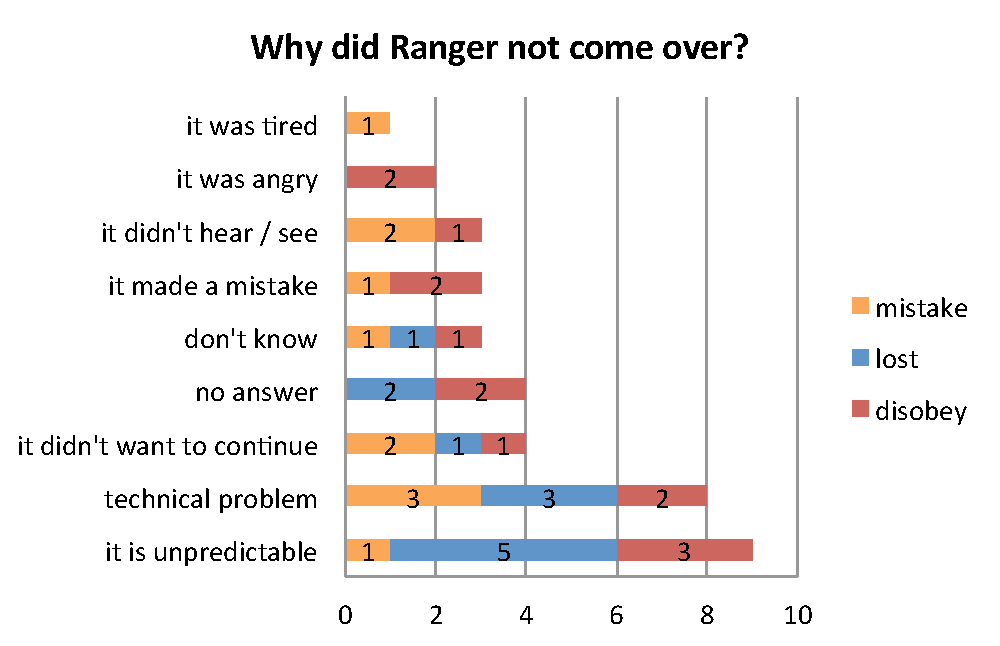
\includegraphics[width=0.8\linewidth]{domino-why-misbehavior.pdf}   
    \caption[Why Did the Robot Misbehave?]{\small Multiple answers were possible
    to the question why the robot did not come over, and we received 37 answers.
    This question shows that children did not necessarily interpret the misbehaviour
    in the way we had assumed.}

    \label{fig:domino-why-misbehaviour}
\end{figure}	

When asked why they thought the robot had not always come
over to them, 4 of the children did not reply. The remaining ones gave a variety
of reasons (Figure~\ref{fig:domino-why-misbehaviour}). The most common answer (9
of 37 replies) was that the robot is somehow \textit{unpredictable} in what it
is doing and that it could go \textit{no matter where}\footnote{We translated
children's answers from French to English. For some expressions the meaning
and connotation of an expression may not be the same. We understand
\textit{``partir dans tous les sens''} as ``to go off in all possible
directions'' and hence interpret this reflects viewing the robot as being
unpredictable.} because \textit{``with robots you have these kind of problems,
they do no matter what''}. 8 replies related to \textit{technical problems}
(including \textit{broken parts}), suggesting that children perceived the
misbehaviour as unintended by the robot. 2 of the children who had interacted
with the disobeying robot said Ranger was \textit{angry}, which none of the
children in other conditions replied. Several children ascribed intentionality
to Ranger explaining that it \textit{did not want to continue} carrying domino
tiles or that it \textit{made a mistake / did something silly}\footnote{We
understood \textit{``faire une bêtise''} as ``to do a silly thing'' in the sense
of making a mistake.}.

Overall, we can notice that not all children perceived the misbehaviour of the
robot as we had intended and we have to keep this in mind while interpreting the
data. Also \cite{leite_long-term_2013} found in her study that when children did
not understand an action of the robot, they tended to view it as a mistake,
rather than interpreting the robot's behaviour as a deliberative action.

%	\textit{``the supportive behaviour ``Play Bad Move'' was not completely
%	understood as a deliberative action of the robot, but rather as a
%	mistake''}. 	

%In our case, it is not easy to make a clear statement about how each of the
%manipulations was perceived by the children.  Similar to how people reacted to
%the cheating robot in the study of \cite{short_no_2010}, most children showed
%surprise, were amused, sometimes confused, or occasionally slightly angry (\eg
%two boys tended to shout to the robot after it had disobeyed). The
%\textit{disobeying} robot seemed to evoke the strongest reactions, partly with a
%negative implication: later three of the children in this condition stated they
%would not accept Ranger as a friend \textit{because it did not always come over
%when they asked it to come over}. \cite{short_no_2010} described a similar
%implication of the robot cheating behaviour: participants made unfavorable
%character attributions to the cheating robot, so the robot's actions affected
%perceptions of the robot as ``fair'' and ``honest''.


%	\cite{short_no_2010} found that participants often had an emotional reaction
%	to the robot's behaviour and made unfavorable character attributions to the
%	cheating robot. The robot's actions affected perceptions of the robot as
%	``fair'' and ``honest''. Qualitatively, the authors found that participants'
%	reactions in the verbal cheat case tended more towards confusion, while
%	their reactions to the action cheat were more exaggerated, showing surprise,
%	amusement, and occasionally anger.  	

%	\cite{short_no_2010} found that participants who saw the action cheat
%	mentioned cheating, while the participants who saw the verbal cheat
%	frequently described it as a mistake or malfunction, while only sometimes
%	calling it cheating.


In terms of \textbf{engagement}, the novelty of the robot certainly plays a role
here. The findings here do not directly address the issues
of long-term usage but concern short-term \textit{engagement}, which is a
pre-requisite for long-term usage.


The huge proportion of \textit{explore} actions (52~\% of all coded actions)
already suggests that children were generally engaged in the interaction, and
most of the time carefully observed what the robot did. When considering the
actions \textit{explore, gesture, look, misuse, show, talk}, and \textit{touch}
as \textbf{engagement actions}, 1699 of the 2354 actions reflected engagement
(72~\%). This indicates that overall children were very engaged in the
interaction with the robot. Furthermore, data suggests that the robot in the
\textit{mistake} and \textit{lost} condition were more engaging for children
(each 75~\% of the actions reflected engagement) than the robot in the
\textit{disobey} condition (66~\% reflected engagement). The statistical
analysis supports this: An ANOVA indicates that there was a significant effect
of robot behaviour on the actions \textit{explore} (F(2,23)=11.31, p<.001) and
\textit{look} (F(2,23)=4.6, p=.021). Post-hoc comparisons using the Tukey's test
indicate that the mean score for \textit{explore} in the \textit{disobey}
condition is significantly different from the score in the \textit{mistake} and
\textit{lost} condition. This suggests that children explored the disobeying
robot less\footnote{It is surprising that the disobeying robot was explored
less. One may expect that the disobeying robot might better attract
children's attention because it faces the searcher child and uses fairly
strong audio and light cues as compared to the other behaviours.}. 

Overall, we found a significant difference between the average of engagement
actions carried out during the first 7 runs (correct robot behaviour) and during
the second 7 runs, when the robot behaved unexpectedly (F(1,36)=5.1, p=.03). In
all three conditions, children carried out more engagement actions with the
unexpectedly behaving robot (Figure~\ref{fig:domino-time-active}). No
interaction effect was found between the two phases of interaction (expected /
unexpected) and condition (F(2,36)=1.2, p=.31). In general, this finding
supports our first hypothesis: children show more engagement toward a robot that
behaves unexpectedly from time to time compared to a robot that always behaves
correctly.

\subsection{Attribution of higher cognitive skills}

\paragraph{Intentionality}

\begin{figure}[h]
    \centering
    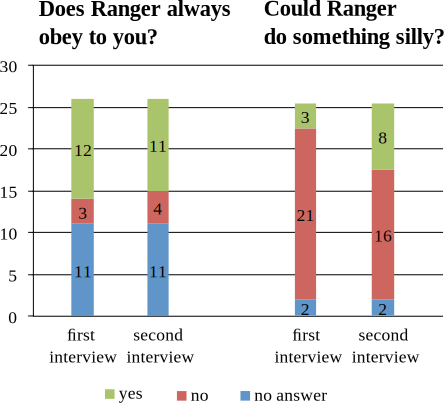
\includegraphics[width=0.75\linewidth]{domino-intention.pdf}
    \caption{\small \textbf{Attribution of intention to Ranger.} Children were
        asked these questions at both interviews. Concerning question (a), there
        are no remarkable differences in children's responses given in the
        \textit{first} and \textit{second} interview.  Children tend to think
        Ranger does always obey to them, even after it misbehaved. There is
        however a small difference in the responses to question (b).  After the
        robot misbehaved, 8 children think the robot could do something silly whereas
        first, only 3 children answered like this.}
    
    \label{fig:domino-intention}

\end{figure}


One of the central points of this study was to investigate to what degree
children attribute intention and cognitive abilities to the robot.  In the first
interview after children had interacted with the correctly behaving robot we
asked three questions to assess how far they ascribe \textbf{intention} to it
(see questionnaire items in Table~\ref{tab:domino-questions}). One of these
questions was whether they believed Ranger could go out the door by itself. The
majority of 16 children answered negatively, which suggests that they initially
do not ascribe intention to the robot. The two other questions were whether
Ranger would always obey and whether Ranger could do a silly thing
(Figure~\ref{fig:domino-intention}). These two questions were asked again later
after children had interacted with the unexpectedly behaving robot.

%	With these recurring questions we wanted to see whether children had changed
%	their mind in terms of ascribing intention to Ranger (and whether the
%	unexpected robot behaviour had caused this effect). This comparison turned
%	out to be difficult, however.  	

Overall, in the first interview 12 of the 26 children believed Ranger does
always obey to them. Asked whether Ranger could do something silly, the great
majority of 21 children replied negatively. We can summarize that after children
had interacted with the \textbf{correctly behaving robot} the majority does
\textbf{not ascribe intention} to the robot.

After they had interacted with the misbehaving robot, we asked children again.
Now, still 11 children (previously 12) believed Ranger would always obey to
them. When analyzing the answers of each child separately, there were 2 children
in the \textit{disobey} condition that changed their answer from \textit{yes} to
\textit{no}; however also 1 child in the \textit{lost} condition that switched
their answer in the opposite way (strangely). There was a more remarkable change
when asking children whether Ranger could do something silly. In the second
interview, 8 children (previously~3) answered Ranger could do something silly. 1
child in the \textit{disobey} condition had changed their answer, and each 2 in
the \textit{mistake} and \textit{lost} condition. 

We can summarize that even with the \textbf{unexpectedly behaving robot}
children do \textbf{not necessarily ascribe intention} to the robot. The
unexpected robot behaviour impacted only some children's attributions of
intention to the robot.  It seemed that some children did not interpret the
robot's misbehaviour as intentional but more like a technical problem or
mistake. For instance, even after the robot misbehaved by \textit{disobeying},
the majority of the children in this condition was still convinced that the
robot could not do a silly thing.  It it interesting to note that children tend
to ascribe cognitive abilities to the robot, like the ability to see and hear
but not intention. We interpret that children may perceive the robot as being
able to process sensory information but that it is not able to make decisions on
its own. 

\paragraph{Emotions}

We examined whether children attributed \textbf{feelings} to the robot by asking
them (once at the end of the experiment) if they thought that Ranger can feel
happy or sad sometimes. The majority of
children (21 of 26) gave a positive answer. Only 2 children who had interacted
with the \textit{disobeying} robot did not believe that Ranger has feelings and
another 3 children (2 \textit{disobey} and 1 \textit{lost}) did not reply at
all. Overall, data suggests that \textbf{children attributed emotional states}
to the robot. Asked for more details, several children answered that it is
through its colors and sounds that the robot shows a feeling. Most children said
that they could make the robot feel happy by playing with it and putting a
domino tile inside the box. This may also be a reflection of their own feelings,
projected on the robot. About half of the children (14 of 26) agreed that Ranger
can be their friend. We did not ask about what being a friend means to them but
as children generally liked playing with the robot, this may be linked to each
other. We can note that children \textbf{ascribe feelings to the robot and
partly accept that it can be a ``friend''}.


\paragraph{Moral standing}

Inspired from the questionnaire used by \cite{kahn_jr._robotic_2006}, we asked
children if it would be alright to leave Ranger alone at home (\eg during two
weeks when they go on a vacation) (Figure~\ref{fig:domino-leave-alone}). 
20 out of 26 children responded negatively. Asked why, children gave a
variety of answers that we classified into 7 categories. With 5 replies, the
most common answer was that the robot ``could do something silly''. Some other
children simply answered they would like to take it with them. Others were
afraid that the Ranger ``would not find its way'' or ``may be taken away by
someone''. 2 children believed Ranger is sad when left alone and 1 child
responded the robot would try to escape. Interestingly, and while we intuitively
expected many children to fear that the robot would be sad if left alone, only 2
expressed a moral position, while most of the others actually expressed several
forms of distrust towards the robot. This shows that things must
be put into perspective and even young children do not automatically consider a
so-called social robot as an actual social agent.

\begin{figure}[!h]
    \centering 
    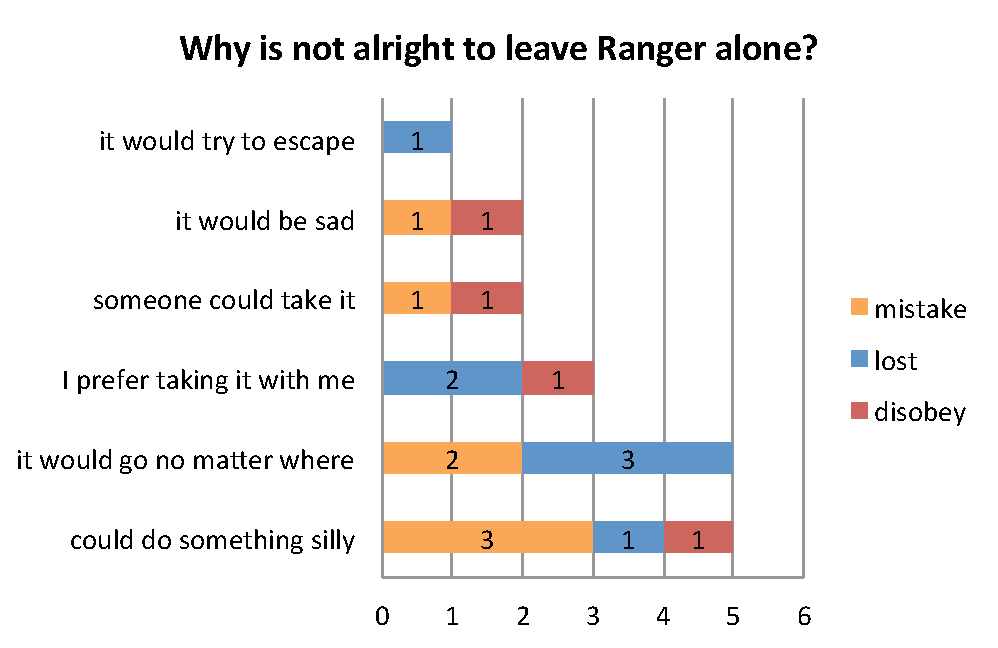
\includegraphics[width=1.0\linewidth]{domino-leave-why.pdf}
    \caption{\small Attributions of moral
        standing: we asked children whether it was alright to leave Ranger
        alone at home if they go on a 2-week vacation. Multiple answers
        (open-ended) were allowed when asked to justify their answer.}

    \label{fig:domino-leave-alone} 
\end{figure}

\subsection{Anthropomorphic projections and social engagement}

The anthropomorphism index expresses to what extent children engaged with Ranger
in a human-like way, both in terms of their behaviour toward the robot and their
perception of the robot. We present here findings on a pair (group) level.

To obtain the anthropomorphism index for a pair, we first calculated the index
per child and then took the average of the two children in one group.  The group
indexes varied between 3.25 and 10.75 points with an average of 7.5 points
(SD~=~2.5), which is 47~\% of the maximum possible index of 16 points.
Intra-group variations were interesting: In 7 of the 13 groups, the
anthropomorphism indexes for both children were similar (difference less than
1.5 points), which means that both children anthropomorphized the robot to a
similar degree. This agreement among children happened for both higher and lower
indexes. In 6 of the 13 groups, the anthropomorphism indexes varied in more than
2 points, which means that one of the children anthropomorphized the robot more
than the other one.

On average, Ranger was moderately anthropomorphized by the
children. 8 of the 13 groups had an index of 8 or higher, evenly spread
over the three conditions (Table~\ref{tab:domino-anth-score}). However, the mean
index of anthropomorphism in the three conditions varied, with the
\textit{mistake} and \textit{lost} condition leading to a higher index than the
\textit{disobey} condition. This finding suggests that the disobeying robot was
less anthropomorphized than the other two robot behaviours, which speaks against
our second hypothesis. We had expected that the disobeying behaviour is
perceived as an intentional action which we assumed would lead to increased
anthropomorphism. This was not the case. The slight difference between the
\textit{lost} and \textit{mistake} robot was also expected in the opposite
direction. It could be that the robot's ``helplessness'' led to this. With the
lost robot, children looked more often at the experimenter than in the other
condition, which suggests that they could not fully make sense of the robot's
behaviour, and the fact of not being able to understand (and hence predict) a
robot's behaviour is likely to increase anthropomorphism.\footnote{One of the
cognitive / psychological explanations for anthropomorphism is that people
want to make sense of something they do not understand and then tend to
anthropomorphize this something (human traits are a good source of making
attributions because this is what people understand best -- themselves and
other humans). For more details the reader may refer to
\cite{epley_seeing_2007}.}

\begin{table}[ht!]
    \centering
    \footnotesize
    \begin{tabular}{lccc}
        \toprule
        & M & SD & groups with index > 8 \\
        \midrule

        \textit{lost} & \textbf{8.31} & 0.59 & 3 of 4 \\ 
        \textit{disobey} & 6.5 & 3.68 & 2 of 5 \\
        \textit{mistake} & 7.94 & 1.74 & 3 of 4 \\ 
        \bottomrule
    \end{tabular}
    \caption{\textbf{Anthropomorphism index.} The maximum possible index was 16. The
    \textit{lost} robot elicits the highest index, which suggests that it is
    anthropomorphized more. Contrary to our hypothesis, data suggests that the
    \textit{disobeying} robot is anthropomorphized less but the \textit{lost} robot
    more.}

    \label{tab:domino-anth-score}       % Give a unique label
\end{table}	

We hypothesized that children who interact a lot and are probably more engaged
with the robot also perceive the robot as more human-like. Data suggests the
opposite, however. As shown in Figure~\ref{fig:domino-anthropo-interaction}, we
found a significant \textit{negative} correlation between the count of
engagement actions (per group) and the qualitative anthropomorphism index
(r(11)=-0.56, p=.05).

%	(b=-.05, t(11)=-2.22, p=.048). 

The overall model with the count of engagement actions (per group) predicts a
significant proportion of the qualitative anthropomorphism index (adjusted
R$^2$=.25, F(1,11)=4.9, p=.05). This means that the more a group showed
engagement in the interaction, the less they anthropomorphized the robot. This
is a key results, which was against our initial assumption. A possible
interpretation is that children who interact more with the robot understand better
how it works, they are more familiar with it, and as such the robot appears less
``mystical'' to them, so there is not a big need to anthropomorphize it. On the
contrary, the cluster of groups that do not interact much but anthropomorphize
the robot more, is quite homogeneous. The negative correlation between the
number of engagement actions and the anthropomorphism index suggests that
children who interact more with the robot tend to anthropomorphize it less. This
implies that anthropomorphism could fade out after some time (or rather after
some interaction). This evokes the question how far anthropomorphism (as a
special kind of social engagement) really helps in sustaining interaction. This
is a critical point because most of the short-term investigations suggest that
anthropomorphic design and human social cues emitted by a robot foster
engagement and acceptance. What if this is not true for continued interaction,
and thus for the long-term?  We have to be careful about our interpretation, due
to the small sample size with which we obtained these findings. We suggest to
investigate the aspect further in future research.

\begin{figure}[t]
    \centering
    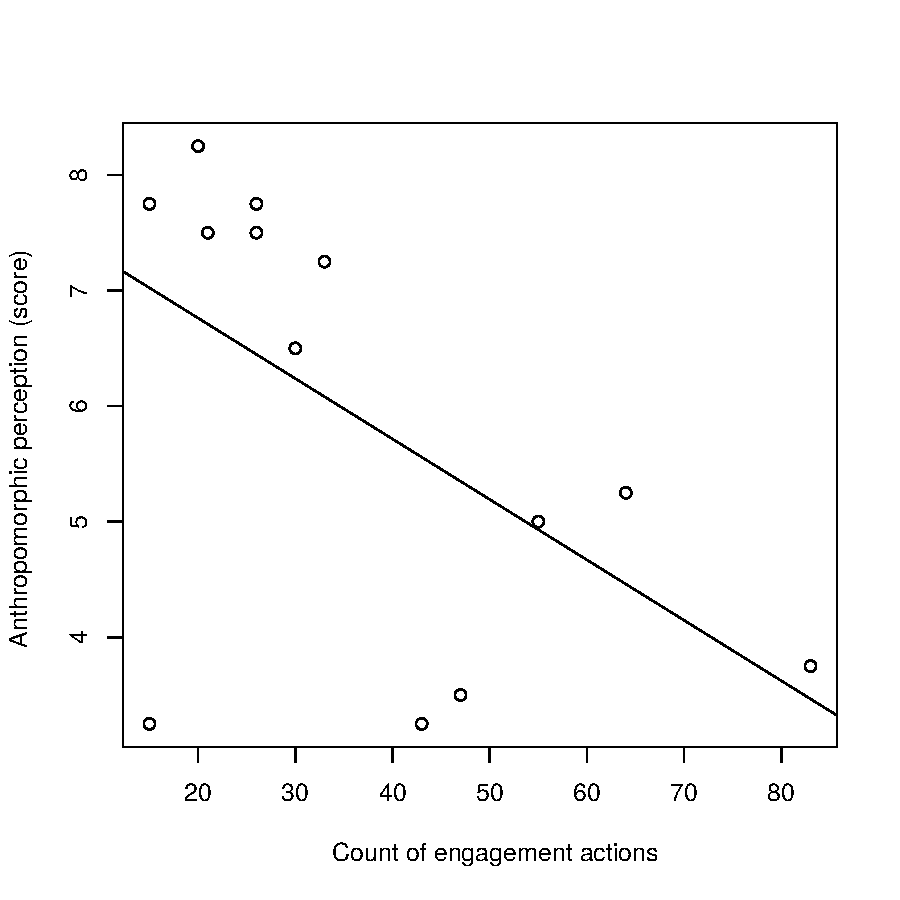
\includegraphics[width=0.7\columnwidth]{domino-correlation.pdf}   

    \caption[Correlation of Anthropomorphic Perception of the Robot and
    Interaction]{\small \textbf{Correlation of anthropomorphic perception of the
    robot and engagement actions.} A scatter plot of the count of engagement
    actions (without explore) and the \textit{anthropomorphic perception} (score per
    group) shows a negative correlation. The score for the anthropomorphic
    perception (\textit{y-axis}) does not take into account the behavioural aspect of
    the anthropomorphism index, as this is part of the interaction
    (\textit{x-axis}).  There seem to be two clusters of groups: those who interact
    more with the robot and anthropomorphize it less, and those who interact less
    but anthropomorphize the robot more.}

    \label{fig:domino-anthropo-interaction}
\end{figure}	

%Our data on the anthropomorphism index also suggest \textbf{qualitative gender
%differences} in children's tendency to anthropomorphize Ranger. Boys (M=8.2,
%SD=3.0) obtained a higher mean index of anthropomorphism than girls (M=6.4,
%SD=2.4). (Interestingly, as it was mentioned before, boys interacted slightly
%more with the robot than girls; though not significantly. This is
%counter-intuitive concerning the negative correlation between amount of
%interaction with the robot and anthropomorphism tendency.) It would be
%interesting to investigate in more detail whether boys are more prone to
%anthropomophize a robot than girls.\footnote{Findings presented in
%\cite{schermerhorn_robot_2008} suggested similar gender differences. In their
%study, males tended to think of the robot as more human-like and accordingly
%showed more ``social facilitation'' than females, who perceived the robot as
%more machine-like.} 


%%%%%%%%%%%%%%%%%%%%%%%%%%%%%%%%%%%%%%%%%%%%%%%%%%%%%%%%%%%%%%%%%%%%%%%%%%%%%%%%%%%%
%%%%%%%%%%%%%%%%%%%%%%%%%%%%%%%%%%%%%%%%%%%%%%%%%%%%%%%%%%%%%%%%%%%%%%%%%%%%%%%%%%%%
\section{Conclusions and Future Directions}


As hypothesised, we found that in a playful scenario where 4-5 year old children
play domino together with a robot, the robot seems to be more engaging when it
shows some misbehaviour compared to when it always behaves as expected
(notwithstanding the likely impact of a novelty effect).

Regarding the design of our three conditions (\emph{lost},
\emph{disobey}, \emph{mistake}), we cannot conclusively affirm whether children perceived the
unexpected robot behaviour as a malfunction (something that happens to a
machine) or as being intended and based on a motivation (something related to a
social entity). Children stated both, when asked why the robot had misbehaved.
Some referred to \textit{``a technical problem''} while others said the robot
\textit{``is tired''} or it \textit{``doesn't want to carry domino tiles any
more but rather go on a tour outside''}. While our manipulations were not as
clearly designed as we expected for the age range of the subjects, we still
believe these three conditions (mechanical malfunction -- the \emph{lost}
condition, vs. explicit intentionality -- the \emph{disobey} condition, vs.
implicit intentionality -- the \emph{mistake} condition) are relevant and we
suggest to replicate a similar study with slightly older children.


%It also appears
%From what we
%have seen in the Domino Study, we have a rough estimate of how children react
%and relate to a robot that behaves unexpectedly from time to time. They are
%mostly surprised, laugh at the robot, and they tend to be more engaged and
%playful. However, they are also confused and cannot really make sense of the
%robot's strange behaviour. We also cannot conclusively tell apart whether children perceived
%the unexpected robot behaviour entirely as a malfunction (something that happens
%to a machine) or as being intended and based on a motivation (something related
%to a social entity). Children stated both, when asked why the robot had
%misbehaved. Some referred to \textit{``a technical problem''} while others said
%the robot \textit{``is tired''} or it \textit{``doesn't want to carry domino
%tiles any more but rather go on a tour outside''}. Maybe our manipulations were
%not as clearly designed as we expected. There is always some freedom in how
%things are interpreted -- especially with young children.  Certainly more work
%needs to be done to investigate which robot behaviour is most beneficial for
%young children and can promote their engagement and motivation to interact with
%Ranger over extended periods of time.  


%	Whereas a cheating opponent is acting out of a desire to win the game, a
%	malfunction, on the other hand, is entirely accidental, and could be the
%	fault of physical design or faulty programming, and can even occur entirely
%	without involvement on the part of the robot. \textit{``A malfunction is
%	something that happens to a machine, while a social entity that can cheat
%	has motivations and desires.'' Short et al.}


%\subsection{Limitations}
%
%This study and the results have several limitations.  First, we did not have a
%real control group in which the robot always behaved correctly. Instead, we took
%the first interaction phase as a reference for how children interact with the
%correctly behaving robot.  Also, the sample size of 13 groups was small. There
%were  variations in the data due to the individual differences of children. More
%data could have allowed for a better comparison between the conditions.
%
%With the manipulation of the robot behaviour we were able to surprise children.
%However, it is questionable how often the same type of behaviour manipulation
%leads to surprise. Moreover, our experiment was a short-term interaction study
%while we try to make statements about how to sustain long-term engagement. This
%is critical but not unusual. Long-term HRI studies with young children are
%extremely rare as they are difficult to set up as well as time and resource
%consuming \cite{leite_long-term_2013}. Nevertheless, we could have probably
%improved our study by setting up several short interaction sessions spreading
%over several weeks. At the end of each session we could have asked whether
%children want to play again with the robot. Such a study could have helped to
%investigate the long-term interaction with the robot and the impact of the
%behavioural variances.
%
%\subsection{Lessons Learned}
%
%One of the lessons learned is that it is difficult to set up a controlled lab
%study with young children. Children are not like adults who patiently
%participate in a 45-minutes experiment and then get some reward in the end. On
%one hand, an experiment with children should not be boring for them, but on the
%other hand, you would like to seriously collect some data. A lot of the
%challenges we experienced are also described in \cite{ros_child-robot_2011}. One
%of the most difficult parts turned out to be the interviews with the children.
%We need to be careful to not over interpret some of their answers. Some children
%seem to not have a clear opinion and partly contradict themselves. These answers
%are not easy to interpret. An interview script including the questions need to
%be designed very carefully, and should definitely be tested beforehand with the
%respective age group.
%
%Overall, it appears that when trying to study something in more detail, such as
%the manipulation of robot behaviour, 4-5 year old children may be too young. But
%when trying to evaluate a more general approach, the design of a prototype, or
%an interaction scenario, children are a very good choice. They say things as
%they are and react very naturally, when compared to adults, who may reply more
%socially desired. 
%
%
%\paragraph{Summary}

%In this study, we investigated the effect of unexpected robot behaviour on
%children's engagement in interacting with Ranger and on their perception of the
%robot.  Our first hypothesis finds support: children show more engagement toward
%a robot that behaves unexpectedly from time to time. Further, different types of
%unexpected behaviour may have a different effect, and therefore the behaviour
%manipulation needs to be designed with care.

Still, we did not find support for our second hypothesis which stated that children
perceive a robot showing intention or cognitive abilities as more human-like
than a robot that appears to have a system error. While this may be due to the study
setup and the fact that children did not interpret the robot misbehaviour in the
conceived way, our findings seem to suggest the contrary to our hypothesis. A
robot that appeared to do a \textit{mistake} or to be \textit{lost} was more
anthropomorphized than a robot that \textit{disobeyed}.


Another outcome of this study is the initial application of an
anthropomorphism index to a child-robot interaction study. This index
considers both behavioural and phenomenological aspects and is able to indicate
lower and higher levels of anthropomorphism along this continuous index.  Our
experience with this index suggests that children tend to conditionally
anthropomorphize the robot. Higher indexes of anthropomorphism were found in the
\textit{lost} and \textit{mistake} condition which was against our hypothesis.

Interestingly, data suggests a significant negative correlation of engagement
and anthropomorphism index. It appears that groups who interacted more with the
robot perceived it as less human-like. This raises an important question for the
human-robot interaction community: to what extent anthropomorphic perceptions
impact the interaction experience. Our findings here go against the intuition.


%%%%%%%%%%%%%%%%%%%%%%%%%%%%%%%%%%%%%%%%%%%%%%%%%%%%%%%%%%%%%%%%%%%%%%%%%%%%%%%%%%%%
%%%%%%%%%%%%%%%%%%%%%%%%%%%%%%%%%%%%%%%%%%%%%%%%%%%%%%%%%%%%%%%%%%%%%%%%%%%%%%%%%%%%
\section*{Acknowledgments}

This research was supported by the Swiss National Science Foundation through the
National Centre of Competence in Research Robotics.

%%%%%%%%%%%%%%%%%%%%%%%%%%%%%%%%%%%%%%%%%%%%%%%%%%%%%%%%%%%%%%%%%%%%%%%%%%%%%%%%%%%%
%%%%%%%%%%%%%%%%%%%%%%%%%%%%%%%%%%%%%%%%%%%%%%%%%%%%%%%%%%%%%%%%%%%%%%%%%%%%%%%%%%%%
\bibliographystyle{abbrv}
\bibliography{domino}

\balancecolumns

\end{document}
